\documentclass{article}
\usepackage[utf8]{inputenc}
\PassOptionsToPackage{hyphens}{url}
\usepackage[colorlinks = true,
            linkcolor = blue,
            urlcolor  = blue,
            citecolor = blue,
            anchorcolor = blue]{hyperref}
\usepackage{graphicx}
\usepackage[section]{placeins}
\usepackage{float}
\usepackage[utf8]{inputenc}
\usepackage{multirow}
\usepackage{csquotes}
\usepackage{xcolor}
\usepackage{amsmath}
\usepackage{longtable}
\usepackage[T1]{fontenc}
\usepackage[normalem]{ulem}
\useunder{\uline}{\ul}{}

\title{Dementia}

\begin{document}

\maketitle

\tableofcontents

\section{Data Sources}
\subsection{Datasets Used}
The datasets used are from the following dementia surveys conducted in Lebanon:
\begin{itemize}
    \item Bekaa Questionnaire: This dataset is the most recent survey conducted last year in the Bekaa. This dataset involved 219 elderly.
    \item full validation data: This data consists of 281 rows. This is the very first survey that we implemented for the sake of testing the 1066 Dementia SPSS algorithm. This survey was conducted on a 1-1 ratio with clinically diagnosed demented patients.
    \item dementia data 502 baseline updated: This is the second survey implemented which involved 502 elderly people. The selection of elderly to participate in this survey was random.
\end{itemize}
We then merged this dataset into one dataset consisting of a total of 1024 elderly.

\subsection{Dementia Output}
In order to label each row (elderly) as positive (has dementia) or negative (does not have dementia), we run the 1066 Dementia SPSS algorithm on our dataset. The result was a total of 1024 patients, 203 of whom have dementia according to the SPSS algorithm.

\section{Split Into numeric and textual}
We have split the data into two chunks, one containing numeric features and another containing categorical features. The Bekaa and full validation questionnaires involved textual questions as well. However, these textual questions are not used by the dementia 1066 SPSS algorithm in determining whether the elderly has dementia or not, so we dropped these textual features from the analysis.

\section{Numeric Features}
\label{sec:numeric}
Our data is now a mix of numerical and categorical features. For the numeric features, we have obtained the following information:
\begin{itemize}
\item \textbf{data type:} Type of the numeric feature. Could possible be: 
\begin{enumerate}
\item \textbf{numeric} meaning this feature has continuous range of values

\item \textbf{categorical} meaning this feature has only a finite set of values, each resembling a specific category

\item \textbf{ordinal} meaning, this feature's values are categorical, but they can be compared between each other. Example would be: a job, were a specific job might be values more than the other. Example: manager vs assistant
\end{enumerate}

\item[] the specification of the \textbf{data type} of each feature was done manually by looking at the range of values in each, and also by looking at the \textcolor{blue}{choices workbook in the copy of dementia Excel questionnaire}

\item \textbf{Description:} Description of each feature

\item \textbf{cat\_options:} Short for "categorical options". \textit{In case the feature is categorical}, what are the possible categories.

\item \textbf{val\_range:} Short for "values range". \textit{In case the feature is numerical}, what are the range of values this feature takes

\item \textbf{min:} \textit{In case the feature is numeric}, what is the minimum value it has

\item \textbf{max:} \textit{In case the feature is numeric}, what is the maximum value it has

\item \textbf{distribution:} link to the distribution plot of each feature on bitbucket. The distribution plot helps in detecting erroneous data

\item \textbf{perc\_missing:} Short for "percentage of missing values". This helps us ggregate features with high percentage of missing. In case the percentage of missing is very high, Imputation methods won't aid much

\item \textbf{perc\_erroneous:} Short for "percentage of erroneous values". Detecting erroneous values was done manually for each feature. Anomalies cover uni-intentional or intentional erroneous values. Example would be having "age" feature being 1966 instead of the actual age

\item \textbf{erroneous:} What were the erroneous values, if any

\item \textbf{cut\_off:} The cut off used to decide whether a feature's value is erroneous or not. The cut off was discovered manually by us for each feature.

\item \textbf{color code:} a color code was applied to each feature to determine whether it belongs to the informant or not.
\end{itemize} 

\subsection{Informant and High Percentage of Missing}
Most of the features associated with very high percentage of missing were directed to informants and related to the living conditions of the family, the house, income, cor-residents of the elderly, etc... which are not used by the SPSS algorithm to label the patients as demented or not (since they are not about the patients) For this reason, we dropped the questions that were about the household, informants, and co-residents

* informant is usually the caregiver of the interviewed elderly person

\subsection{Nested Questions and High percentage of missing}
Since our data is survey in nature, some features are actually questions are related to the other. If a certain question is asked to the elderly, and only based upon the elderly's answer, the interviewer might ask the elderly another question or not. Let us give an example:
\begin{enumerate}
\item the interviewer asks if there has ever been a period when the elderly smoked cigarettes, cigars, a pipe, or water pipe nearly every day?

\item \textbf{Only if the answer to the question above was a Yes}

\item the interviewer asks the following questions:
\begin{enumerate}
\item What did the elderly smoke?
\item How old were you when you started using tobacco regularly? (if the above is true)
\item Do you still use tobacco regularly?
\end{enumerate}
\end{enumerate}

We also realized that many features have high percentage of missing because a parent question's answer did not cause a jump to that feature question.


\subsection{Treating Features with High Percentage of Missing}
\label{sec:legalizingfeatures}
We divided the features as follows:
\begin{enumerate}
\item \textbf{Informant} A feature belongs to this category if the question is asked to the informant

\item From Informants we have:
\begin{enumerate}
\item \textbf{parent} Questions that caused jumps to other questions

\item \textbf{child} child of parent question
\end{enumerate}

\item \textbf{Non-Informant}
We also have:
\begin{enumerate}
\item \textbf{parent}
\item \textbf{child}
\end{enumerate}
\end{enumerate}

We followed the following steps in order to eliminate features with high percentage of missing:
\begin{enumerate}
\item remove all informants and their children questions (so we removed all informants, and if one of them happens to be a parent question, we removed all its children questions)

\item It is important to note that all parent questions informants have their children questions also informant

\item Then we are left with \textbf{Legal features}

\item From legal features, remove all children
\end{enumerate} 

\textbf{\textit{After doing the steps above, the number of \textcolor{blue}{numerical features} decreased from 542 to 257, all of which have 0\% missing (with the exception of 1 feature whcih has 50\% missing)}}

\subsection{Detecting Erroneous Values Inside Features}
In our dataset, the categorical and ordinal values are encoded with numbers ranging from 1 to the length of the categories. therefore, since our categorical, ordinal, and numerical values are all numbers, we set cut-offs to determine erroneous values. 
For some of the features, the erroneous values are straight forward to detect, based on the description for the question. These are the following:
\begin{itemize}
    \item age: some people enter the year, others enter the age. for this, if the value of both the numb as is or 2020 - the numb is more than 100, this means that the person is more than 100 years old which renders the age erroneous. For age, the cut-off was 100
    \item helphour: number of hours per week the elderly needed help, therefore bounded by max numb of hours in a week
    \item learn questions: the patient is supposed to repeat 3 words, bounded by the max numb of words: 3
\end{itemize}
For the rest of the categorical and ordinal values, we get the maximum number encoding for the question options from the options excel sheet based on which the interviewers selected these options. The cut-off is therefore the maximum number encoding a category. Were therefore label any value that is greater than the cut-off to be erroneous.

\subsection{Working with Legal Features}
As mentioned in section \ref{sec:legalizingfeatures}, the remaining \textbf{\textit{"Legal"}} Features are the 257 out of originally 542. We will be using these 257 \textbf{\textit{"Legal"}} features as input for data pre-processing and cleaning techniques.

\subsection{Filtering Legal Features with Erroneous Values - Erroneous Code-Book}
In section \ref{sec:numeric}, we talked about how some of the 542 numeric features have erroneous values. However, as we will be working with only "Legal" features, its important to filter out which subset of the features with erroneous values are actually "Legal". Thats's why, we did the following:

\begin{enumerate}
    \item From all the features containing erroneous, filter out the ones that are Legal
    \item From the Legal ones:
    \begin{enumerate}
        \item get the feature name
        \item get the feature's description
        \item get the feature's percentage of erroneous values
        \item get the feature's actual erroneous values
        \item Display the feature's cut-off on values which decides which values are erroneous (crossing the cut-off) and which are non-erroneous (not crossing the cut-off)
    \end{enumerate}
    \item When done from 2. above, sort the features by decreasing order of percentage of erroneous values
\end{enumerate}

\subsection{Detecting Outliers}
We want to investifgate the existsence of outliers in the data. We have 3 different data types:
\begin{enumerate}
    \item \textbf{Numeric}: very few columns
    \item \textbf{Ordinal}: categorical values that obey a certain order of importance
    \item \textbf{Categorical}
\end{enumerate}

\noindent The outlier detection methods are known for numeric values, but it is \textbf{ordianl} and \textbf{categorical} values that raise the question of how are we going to detect outliers with such types of data ?

\noindent We will assume that ordinal values are numeric. We will prove the legit-ability of our assumption through an example:

\noindent Assume for instance, that we have a column that shows the socio economic status (“low income”,”middle income”,”high income”), education level (“high school”,”BS”,”MS”,”PhD”), income level (“less than 50K”, “50K-100K”, “over 100K”), satisfaction rating (“extremely dislike”, “dislike”, “neutral”, “like”, “extremely like”). These are not categorical but rather ordinal, and if we give, for example, the income level the following labels:
\begin{itemize}
    \item less than 50K: 0
    \item 50K-100K: 1
    \item over 100K: 2
\end{itemize}
Then it is definitely the case that 2 $>$ 1 $>$ 0. And if we have an individual who earns, $>$ 1000 K, we give this the label 3, and these individuals are definitely rare and can be considered as outliers

\subsection{Outlier Detection and Scaling}
We try different scaling methods before we detect outliers, and we apply the outlier detection only for columns \textit{that are: numeric and/or ordinal}, and we extracted the percentage of outliers for each of the legal columns as well as the outlier values themselves (values considered outliers).

\noindent We realize that the outlier values, for the \textbf{ordinal} columns, happen to be the values \textit{8 and 9} which is normal because the values are either 0,1,2 or 8,9.

\subsection{Feature Cross}
Our data mostly consists of categorical/ordinal columns, and we have to find a way to solve these non-linearities such that it fairs better for the model's understanding of the features when we begin with the modelling phase. We generate the list of all possible feature crosses. 

\noindent Feature crossing, will come after we 'one-hot encode' our data.


\section{Feature Selection}
\subsection{Decision Tree Feature Importance}
We use decision trees to calculate feature importance implemented using scikit-learn's DecisionTreeRegressor.

After being fit, the model provides a feature\_importances\_ property that can be accessed to retrieve the relative importance scores for each input feature.

The results of the feature importance using the dummy imputed pooled data so far is then stored in the 'feature\_importance.csv', sorted from highest (highest importance score) to lowest (lowest importance score).

\subsubsection{Select K Best Features}
\subsubsection{Deciding "K"}
In order to select K best features, we need to first decide the value of K. In order to do this, we use sklearn's RFECV, which uses step forward recursive feature elimination and cross validation to decide the number of features needed to give the highest out of sample accuracy.
\subsubsection{Selecting K Best Features}
After deciding on the value of K, which using the current imputation of the input data turned out to be 20, we perform step forward recursive feature elimination that ranks all the features as 0 or 1, with 1 meaning that a feature is one of the K best features. We store the names of the k-selected features (column names) into a csv file called "k\_best\_features.csv"

\section{Oversampling and Undersampling}
Based on the examples discussed in the books, we implemented 4 functions that accept a model and add it to a pipeline after adding the oversampling/undersampling layers. The following are the functions created:

\begin{enumerate}
    \item random\_sampling: consists of a random oversampling and a random undersampling layers
    \item smote\_random\_sampling: adds a smote oversampler and a random undersampler
    \item smote\_tomek (combination approach): combines over and under sampling using SMOTE and Tomek links.
    \item smote\_enn: combines over and under sampling using SMOTE and Edited Nearest Neighbours
\end{enumerate}

\section{Chapter 6: Precision, Recall, and F-measure}
The chapter summarizes the precision, recall, and f-measures of multiclass and binary classification for the case of balanced data.

\section{Chapter 7:ROC Curves and Precision-Recall
Curves}
ROC Curves (receiver operating characteristic curve) and ROC AUC (area under the ROC curve) are used to decide if the model differentiates between the labels. 
\subsection{ROC Curve}
The threshold is applied to the cut point in probability between the positive and negative classes. In order to decide on the best threshold, we evaluate the true positive and false positives for different threshold values, a curve can be constructed that stretches from the bottom left to top right and bows toward the top left. This curve is called the ROC curve. A classifier that has no discriminative power between positive and negative classes will form a diagonal line between (0,0) and (1,1). Models represented by points below this line have worse than no skill.
\subsection{AUC}
Area under the curve is calculated to give a single score for a classifier model across all threshold values. This is called the ROC area under curve or ROC AUC or sometimes ROCAUC. The score is a value between 0.0 and 1.0, with 1.0 indicating a perfect classifier.
\section{Chapter 8: Probability Scoring Methods}
\subsection{Probability Metrics}
On some problems, a crisp class label is not required, and instead a probability of class membership is preferred. The probability summarizes the likelihood (or uncertainty) of an example belonging to each class label. 
\subsection{LogLoss Score}
Logarithmic loss or log loss for short is a loss function known for training the logistic regression classification algorithm. The log loss function calculates the negative log likelihood for probability predictions made by the binary classification model. Most notably, this is logistic regression,but this function can be used by other models, such as neural networks, and is known by other names, such as cross-entropy.
\section{Cross Validation for Imbalanced Datasets}
The solution is to not split the data randomly when using k-fold cross-validation or a train-test split. Specifically, we can split a dataset randomly, although in such a way that maintains the same class distribution in each subset. This is called stratification or stratified sampling and the target variable (y), the class, is used to control the sampling process. This is available using sklearn stratified kfold.
\section{Chapter 10}
Summarizes oversampling and undersampling techniques which are available in chapters 12 and 13 in details.
\section{Chapter 12}
\subsection{Oversampling}
All techniques available through the python library: imblearn.over\_sampling

\begin{itemize}
    \item Random Oversampling: simplest oversampling method, involves randomly duplicating examples from the minority class in the training dataset
    \item SMOTE (Synthetic Minority Oversampling Technique): works by selecting examples that are close in the feature space, drawing a line between the examples in the feature space and drawing a new sample as a point along that line
    \item Borderline-SMOTE: involves selecting those instances of the minority class that are misclassified, such as with a k-nearest neighbor classification model, and only generating synthetic samples that are difficult to classify. Borderline Oversampling is an extension to SMOTE that fits an SVM to the dataset and uses the decision boundary as defined by the support vectors as the basis for generating synthetic examples, again based on the idea that the decision boundary is the area where more minority examples are required.
    \item Adaptive Synthetic Sampling (ADASYN): another extension to SMOTE that generates synthetic samples inversely proportional to the density of the examples in the minority class. It is designed to create synthetic examples in regions of the feature space where the density of minority examples is low, and fewer or none where the density is high.
\end{itemize}
\subsection{Undersampling Techniques}
\begin{itemize}
    \item Random Undersampling
\end{itemize}
\section{Data Transforms (Hiyam)}
\subsection{Scaling Numeric Data (chapter 17)}
\begin{itemize}
\item Normalization (Min-Max Scaling)
\item Standardization
\end{itemize}

\subsection{Scaling Data with Outliers (chapter 18)}
Many machine learning algorithms perform better when \textbf{numerical} input variables are scaled. Standardization is a popular scaling technique that substracts the mean from the values and divide by the stadard deviation, transforming the probability distribution from for an input variable to a Standard Gaussian (zero mean and unit variance).

\noindent \textbf{Problem:} Standardization can become skewed or biased when the input variable contains outliers.

\subsubsection*{Robust Scaling}
When we are scaling the data, and if we have very large values relative to the other input variables, these large values can dominate or skew some machine learning algorithms. \textbf{The result is that the algorithms pay most of their attention on the large values and ignore the variables with smaller values}.

\noindent Outliers are values at the edge of the distribution that may have a low probability of occurence, yet are overrepresented for some reason. \textbf{Outliers can skew a probability distribution and make data scaling using standardization difficult as the calculated mean and standard deviation will be skewed by the presence of outliers.}

\noindent \textbf{Approach:} When standardizing input variables containing outliers, we can ignore outliers from the calculation of the mean and standard deviation, and use the calculated values to scale the data

\noindent \textbf{This is called robust standardization}. This can be achieved by calculating the median (50th percentile) and the 25th and 75th percentile. The values of each variable can then have their median subtracted and are divided by the inter quartile range (IQR) which is the difference between the 25th and 75th percentile.

\begin{equation}
value = \frac{value - median}{p_{75} - p_{25}}
\end{equation}

The resulting value has a \textbf{zero mean and median and a standard deviation of 1}. Although not skewed by outliers and the outliers are still present with the same relative relationships to other values.

\subsection{How to Encode Categorical Data (chapter 19)}
Machine learning models require all input and output variables to be numeric. This means that if the data contains categorical data, we must encode it to numbers before we fit and evaluate our models.

\subsection*{Ordinal Encoding}
Each unique category is assigned an integer value. Example: \textit{red} is 1, \textit{green} is 2, \textit{blue} is 3.

\noindent For categorical variables, it imposes and \textbf{ordinal relationship} when no such relationship exists. This may cause problems and \textbf{one hot encoding} may be used instead.

\subsection*{One Hot Encoding}
For categorical variable where no ordinal relationship exists, the ordinal encoding is not enough and may be misleading.

\noindent One Hot Encoding works by creating binary variables for each category. For Example: \textit{red} will be [1, 0, 0], \textit{blue} will be [0, 1, 0], and \textit{green} will be [0, 0, 1].

\subsection*{Dummy Variable Encoding}
The one hot encoding includes a binary representation for each category. This might cause redundancy. 

\noindent if we know that [1, 0, 0] represents \textit{blue}, and [0, 1, 0] represents \textit{green}, we don't need another binary variable to represent \textit{red}, instead we could use 0 values along, e.g. [0, 0]. This is called dummy variable encoding and always represents $C$ categories with $C-1$ binary variables.

\noindent Other being less redundant, it is required for some models.

\subsection{How to Make Distributions Look More Gaussian (chapter 20)}
Several Machine Learning Algorithms assume the numerical values have a Gaussian distribution. Our data may not have a Gaussian distribution and it might have a Gaussian-like distribution.

\section{Data Pre-Pocessing}
After we have filtered the legal features in our data, and we deleted the features that have $>$ 40 \% missing values, we are left out with 255 legal features. These features must be pre-processed before we do the modelling exercise, for the following reasons:
\begin{enumerate}
\item All the 255 legal features still have missing values
\item We have a combination of numeric, ordinal, and categorical features, whereby each might require a different kind of scaling
\end{enumerate}

\subsection{Imputation in Ordinal/Categorical Data}
To be continued ... waiting to meet with Dr Khalil again. Some notes:
\begin{enumerate}
    \item We said we might do KNN and impute by getting the values from the nearest neighbors.
    \item It is common that public health practitioners usually disregard features with greater than 25\% missing, and since we have features that have greater than 25\% missing, we got the \textbf{theme} of each feature, and if the feature belongs to a particular theme that might not be of vital importance for detecting dementia, we will dis-regard the feature by itself.  
\end{enumerate}

\subsection{Imputation Currently Done}
Just for now, to get things going, we imputed all missing values by replacing with the majority

\subsection{Scaling}
We have said earlier that we have three data types in our features: \textit{\textbf{numeric, ordinal, and categorical.}}

\begin{itemize}
    \item For ordinal and numeric data, we will be using the \textbf{Robust scaling} mechanism due to the presence of outliers
    \item For categorical data, we will not scale it as we will be applying \textbf{dummy variable encoding} 
\end{itemize}


\subsection{Encoding Data}
\begin{itemize}
    \item For ordinal features, we will be applying Ordinal Encoding, as it will maintain an order between feature values.
    \item For categorical features, we apply dummy variable encoding that decreases redundancy of one hot encoding
\end{itemize}





\section{Advanced ML Evaluation Techniques}
In this paper, authors seek to solve the problem of predicting students who are at risk of dropping out of highschool or not. They have a \textbf{binary classification problem} and they predict if the student graduates (0) or does not (1). School principals want to see if they can have enough budget to afford those - \textbf{at an early stage} - that are at risk of not graduating and help them with additional materials. Non-Machine learning practitioners do not value regular evaluation metrics like precision and recall because it means nothing to them, they want some evaluation techniques that could help understand the predictions more from their point of view

\subsection*{Disclaimer}
\begin{itemize}
\item I have read only sections 5 \& 6 from the paper as instructed by Dr. Fatima
\item I have found a github repository for their work here: \url{https://github.com/dssg/student-early-warning} but their work is not complete at all, the only thing that they did - with regards to sections 5 \& 6, is compute the \textbf{\textit{risk}}. The rest of the work is done solely by me. 
\item I used the data they provided in their github repository to complete my work, they also do not provide the complete data and there are differences between the column names mentioned in the paper and the columns in the dataset they provide. But I still worked with this incomplete version of the data 
\end{itemize}

\subsection{Analysis of Predictive Models}
School districts are interested in identifying those students who are are at risk of not graduating high school on time so that plan their resource allocation ahead of time.

\noindent \textbf{Goal:} predict if a student is at \textbf{risk} of not graduating high school on time

\subsection{Evaluation Using Traditional Metrics}
\begin{itemize}
\item We have a binary outcome, use standard evaluation metrics such as \textit{accuracy, precision, recall, f-measure, and AUC}
\item Their data is \textbf{imbalanced}:
\begin{enumerate}
\item \textbf{Class 0: 91.4\%}
\item \textbf{Class 1: 8.6 \%}
\end{enumerate}

\item I must do a \textbf{stratified} split of classes between training and testing such that if the original data has X\% 0s and Y\% 1s, then the training as well as the testing must also have X\% 0s and Y\%  1s

\item I have added \textbf{SMOTE} so that we can \textbf{oversample} our \textbf{training} data before predicting

\item I used MinMax Scaling (just for now because my focus is on the implementation of the ideas in sections 5 \& 6)

\item In this paper they only use shallow models, this what I also do (just for now because my focus is on the implementation of the ideas in sections 5 \& 6)

\item In Figure \ref{Fig:roccurves} below, I show the ROC curves of various models
\end{itemize}

\begin{figure}[H]
\centering
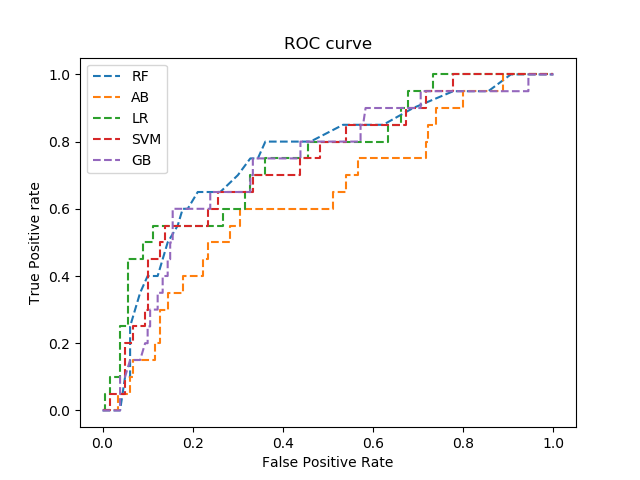
\includegraphics[scale=0.5]{roccurves.png}
\caption{ROC Curves of various shallow models trained on the data provided}
\label{Fig:roccurves}
\end{figure}

\subsection{Problem with Standard Evaluation Metrics}
\begin{enumerate}
\item Educators think about the performance of an algorithm in a slightly different fashion
\item the availability of resources varies with time. For example, a school might support 100 students in 2012, and 75 in 2013. 
\item We want to build algorithms that can cater to these changing settings
\end{enumerate}

\subsection{Solution: Risk Estimates}
\begin{itemize}
\item an algorithm, to cater to their needs, must provide them with a list of students ranked by some measure of \textit{risk} such that, the students at the top of the list are at a higher risk of not graduating on time.

\item Once educators have such a ranked list, they can choose the \textbf{top k} students from it and provide assistance to them

\item \textbf{Challenge:} We only have binary records, but fortunately, all classification algorithms provide internally a probability of each class we have, we can use this probability to derive our \textbf{risk} measure
\end{itemize}

\subsection{Ensuring Quality Of Risk 
Estimates}
\subsubsection{From Models to Risk Estimates}
\begin{itemize}
\item The output of our predictions are binary: either 0 (will graduate on time) or 1 (will not graduate on time)
\item Algorithms allow us to get the  \textbf{probability} of each class. Here, we focus on the probability of the \textbf{positive} class (which shows the probability of not graduating on time). We use the probability of the predictions on the \textbf{final testing data }
\end{itemize}

\subsubsection{Measuring the Goodness of Risk Scores}
\begin{itemize}
\item We first get the probability of not graduating on time (class: 1) for each of the testing instances (students) we have. We call this \textbf{\textit{risk}}

\item Rank the testing instances (students) in descending order of \textbf{risk} estimates. This way, students with higher probability of not graduating on time are at the top of the list.

\item Group students into \textbf{bins (percentiles)} based on their risk scores. We can decide, for example, to choose 10 bins, and when we do, then the students who fall between the 10th and 20th percentile have very little risk scores, those between 20th and 30th have more risk scores than the latter 

\item \textcolor{blue}{My problem with this is as follows: we are doing the 3 bullets above for all the algorithms we have. The distribution of risk scores, for un-balanced classification problems, is usually very skewed and therefore, we can have the following 2 scenarios:}
\begin{itemize}
\item We might not be able to group them into 10 bins for example because each bin must have the same number of instances and that might not be possible in the un-balanced skewed distribution
\item A possible solution to the problem above is to decrease the number of bins.
\item Even if we decrease the number of bins, we might not be able to attain the same number of bins for every algorithm we have. If you look at Figure 2 in their paper, you see that for all algorithms they were able to distribute risk scores into 10 bins, but in case one is not able, we cannot produce such a plot
\item One solution is to distribute them into bins but \textbf{without guaranteeing the same number of instances in each bin  }
\item Even if we are able to produce such a plot, the 10 bins won't be unique (in terms of lower and upper limits) for each algorithm. Is that valid to work with ?  
\end{itemize}
\item For each bin, we produce the \textbf{mean empirical risk} which is the fraction of students, from that bin, who actually (as per ground truth) fail to graduate on time.
\item This curve is called \textbf{mean empirical risk} curve
\item An algorithm is considered to be producing good predictions if its empirical risk curve is \textbf{monotonically non-decreasing} (as the risk scores increase, we have more \textbf{correct} predictions about the positive class (more students who actually - as per ground truth - fail to graduate on time))
\end{itemize}

I present below the empirical risk curve of the shallow models I trained on - \textbf{with incorporating SMOTE} and MinMax Scaling
\begin{figure}[H]
\centering
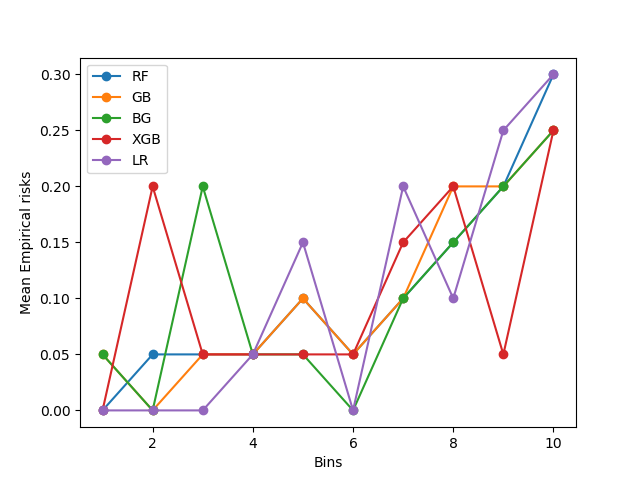
\includegraphics[scale=0.5]{meanempiricalrisks.png}
\caption{Mean Empirical Risks per Model}
\label{Fig:MeanEmpiricalRisks}
\end{figure}

\subsubsection{Comparative Evaluation of Risk Estimates}
It is good to see the models performances on the \textbf{Top K} students \textbf{at risk}. The steps we do to attain this:
\begin{enumerate}
\item Rank Testing instances (students) by their \textbf{risk} scores
\item Define a list of \textbf{K}s
\item For each value \textbf{k} of \textbf{K}:
\begin{enumerate}
\item get the top \textbf{k} predicted values
\item get the ground truth  of these \textbf{top k}
\item compute the precision/recall
\end{enumerate}
\end{enumerate}
\noindent We get the precision and recall at top K and we produce the following curves:

\begin{figure}[H]
\centering
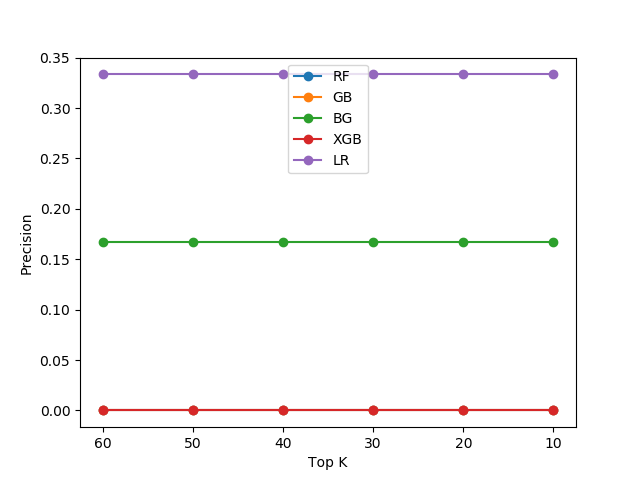
\includegraphics[scale=0.5]{precisionstopK.png}
\caption{Precision at Top K}
\label{Fig:prectopk}
\end{figure}


\begin{figure}[H]
\centering
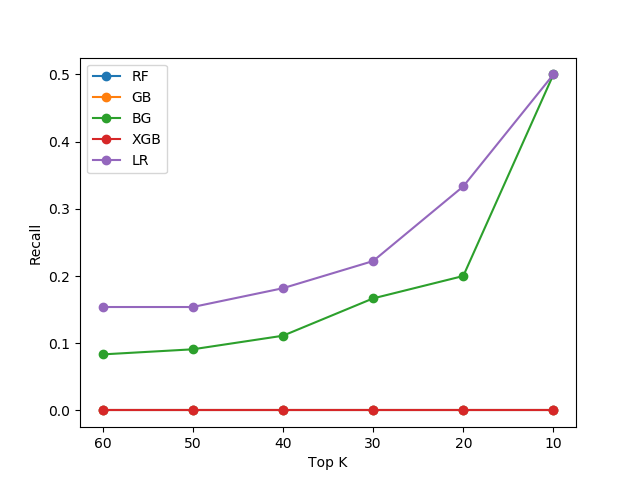
\includegraphics[scale=0.5]{recallstopK.png}
\caption{Recall at Top K}
\label{Fig:prectopk}
\end{figure}

\subsection{Interpreting Classifier Outputs - FP Growth}
\subsection*{Frequent Patterns}
To understand FP Growth algorithm, we need to first understand association rules.

Association Rules uncover the relationship between two or more attributes. It is mainly in the form of- If antecedent than consequent.  For example, a supermarket sees that there are 200 customers on Friday evening. Out of the 200 customers, 100 bought chicken, and out of the 100 customers who bought chicken, 50 have bought Onions. Thus, the association rule would be- If customers buy chicken then buy onion too, with a support of 50/200 = 25\% and a confidence of 50/100=50\%.

\textbf{References:} \url{https://www.mygreatlearning.com/blog/understanding-fp-growth-algorithm/}

\subsection{Technicalities}
\noindent Usually, for identifying frequent patterns, we are represented with a \textbf{transactions} dataset, where each row represents \textbf{a set of items} bought by a customer. \textbf{However, we do not have transaction, we rather have multivariate dataset with a bunch of numerical columns. How can we do it?}

\textbf{\textcolor{blue}{Disclaimer: The methodology below presents my own solution of the problem, I am not able to find such a technique anywhere on the internet.}}

In order to \textbf{present} values as items:
\begin{enumerate}
\item Consider Each column value, in a row, as being an \textbf{item} bought by the customer.
\item Our values are numeric, therefore, to avoid redundancy, I categorize the values as follows:
\begin{itemize}
\item value $<=$ 25th percentile
\item 25th percentile $<$ value $<=$ 75th percentile
\item value $>$ 75th percentile
\end{itemize}
\item Do the categorization above, \textbf{per column}, for all values in the dataset
\item Achieve the so called "Item Dataset" where each row has one item (from the categories generated above) per column
\item Apply the FP-growth Technique on the generated "Item Dataset"
\item Extract the most frequent patterns
\end{enumerate}

The reason I did the aforementioned methodology above is because, in the \textbf{paper we are referencing (montogemery)}, they have frequent patterns like (GPA $>$ 2.0) and (Absence rate $<=$ 0.1), therefore I deduced that these can be taken by doing 'quartiles' of the distribution of values we have per column.

\subsection{Characterizing Prediction Mistakes}
\begin{enumerate}
\item Get all frequent patterns using the methodology I created above that incorporates FP-Growth
\item Rank predictions based on risk score probabilistic estimates

\item Create a new field called \textit{mistake} which is 1 if the prediction does not match ground truth and 0 otherwise

\item \textbf{For each frequent pattern} identify the \textbf{probability of mistake} by computing the number of mistakes done per frequent pattern

\item Do all of the above bullets \textbf{for each model. Therefore, we end up with a probability of mistake for each frequent pattern, per model}
\end{enumerate} 



\subsection{Comparing Classifier Predictions}
When we present educators with a suite of algorithms, they are keen on understanding the differences between \textit{rank orderings} produced by each of these algorithms.

\noindent We will be using \textbf{Jaccard Similarity} for measuring similarity between predictions, \textbf{also at Top K}:

Let's say we have 200 testing instances (students). One model might put the highest risk score for the 180th testing instance, another model might put the highest risk score for the 190th testing instance. Therefore, it is important to note that in this exercise, we find which testing instances were chosen to be in the top k between model 1 and model 2, and we compute, using the jaccard similarity, the intersection of these testing instances (over their union). Good models must have very high intersections if they are classifying instances properly.
 
\begin{enumerate}
\item Get all possible \textbf{combinations} of model pairs (we are using a suite of models)
\item For each model pair, and for each \textbf{k} in \textbf{K}:
\begin{enumerate}
\item get the testing instances at top \textbf{k} from model 1 of the model pair
\item get the testing instances at top \textbf{k} from model 2 of the model pair
\item Compute jaccard similarity as the intersection of the two testing instances from each model over their union
\end{enumerate}
\end{enumerate}

After doing this, we get the following results:
\begin{figure}[H]
\centering
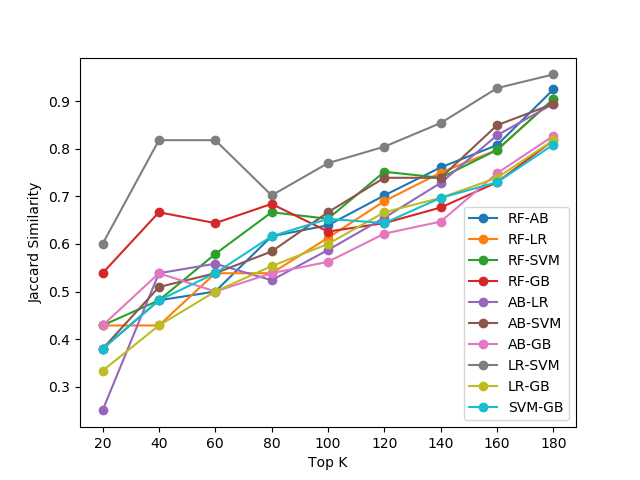
\includegraphics[scale=0.6]{jaccardtopK.png}
\label{Fig:jaccardtopk}
\caption{Jaccard Similarity of students at risk for various algorithms}
\end{figure}


\section{Advanced ML Evaluation of Fake News Experiments}
We have already done the fake news experiments before, and for each experiment \textbf{with the exception of Expriment 2}, we have saved the \textbf{trained models}. We have made our code \textbf{accept trained models}, and assess their performance on \textbf{testing dataset} passed by the user, with the performace asssessed, hereafter, by advanced ML Evaluation techniques presented in this report.

\subsection*{Fake News Repository}
The fake news repository with latest experiments is found here on bitbucket in the latest folder called \textit{Hiyam}: \url{https://bitbucket.org/rba15/fake_news_detection/src/master/Hiyam/} 

\subsection{Experiment 1}
In Experiment 1, we have trained a suit of \textbf{shallow} ML models on the FA-KES training data and tested it on the FA-KES testing data as well. Ofcourse, it is important to note that we have split the original FA-KES data in a \textbf{stratified manner}, hereafter, maintaining the same class distribution between training and testing dataset splits.

\noindent We have chosen the \textbf{number of bins to be equal to 3}. By the number of bins, we mean the bins were the probabilistic risk scores fall in, in ascending order (smaller bins have smaller risk scores; higher bins have higher risk scores)

\subsubsection{Mean Empirical Risks}
\begin{figure}[H]
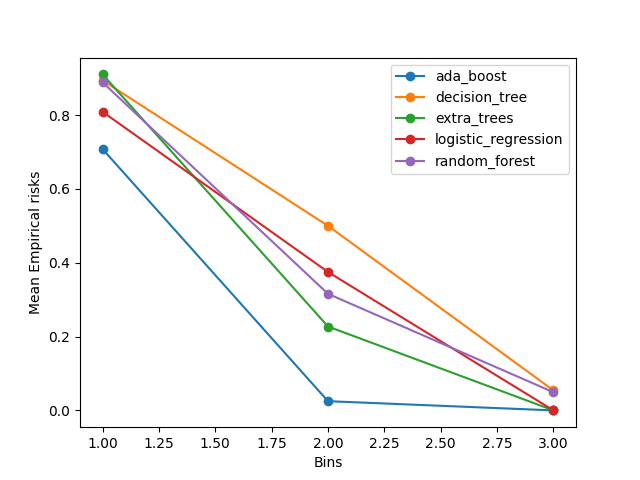
\includegraphics[scale=0.6]{fakeexp1/meanempiricalrisks.png}
\caption{plot that shows the mean empirical risks across the 3 bins}
\end{figure}

\textbf{Unfortunately}, this is not a good plot at all. The mean empirical risk, which defines the mean of the risk scores at each bin, decreases as we get to higher order bins. This is indicative that the models trained on FA-KES and tested on FA-KES are not good at all, they are assigning \textbf{lower risk scores for instances that are actually, as per ground truth, FAKE, and higher risk scores for instances that are actually, as per ground truth, not FAKE}. The trained algorithms are doing a bad job. it is important to note that a good mean empirical risk curve should me monotonically non-decreasing. Here we invert it :) 

\subsubsection{Precision at Top K}
\begin{figure}[H]
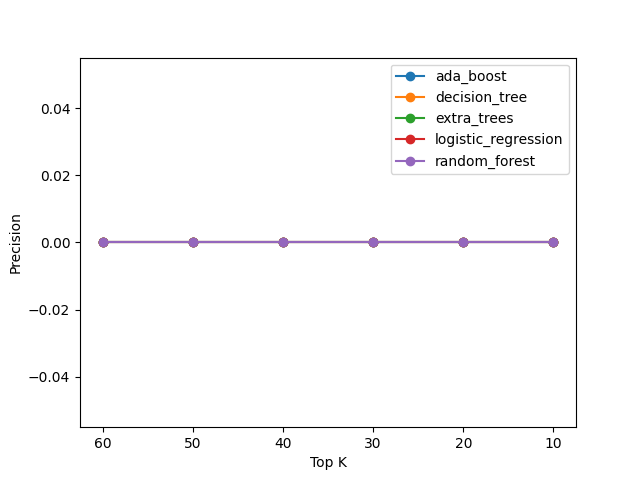
\includegraphics[scale=0.6]{fakeexp1/precisionstopK.png}
\caption{Precison at Top K instances that have the highest risk scores}
\end{figure}
This plot is not good. Something is a bit off as the precision remains at 0 ??

\subsection{Recall at Top K}
\begin{figure}[H]
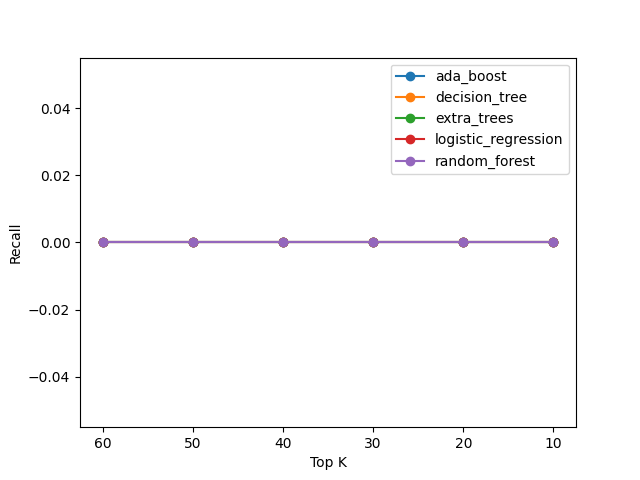
\includegraphics[scale=0.6]{fakeexp1/recallstopK.png}
\caption{Recall at Top K instances that have the highest risk scores}
\end{figure}
This plot is not good. Something is a bit off as the precision remains at 0 ??


\subsection{Jaccard Similarity at Top K}
\begin{figure}[H]
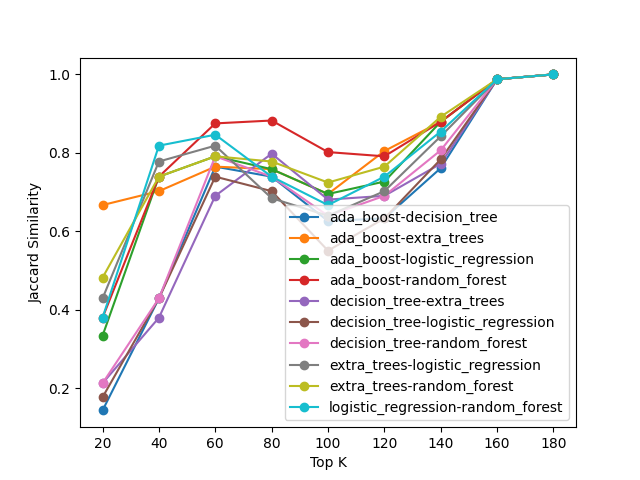
\includegraphics[scale=0.6]{fakeexp1/jaccardtopK.png}
\caption{Jaccard Similarity at Top K instances that have the highest risk scores}
\end{figure}
Some light in this plot. For any given K, the algorithms return the set of K news that are likely to be fake based on the risk scores. Good algorithms must return the same set of K instances that are likely to be fake. 
\noindent We realize that as the number of instances K increases, the similarity between all model pairs increase, with the highest similarity is between the Ada Boost and the Random Forest models.

\subsection{ROC Curves}
\begin{figure}[H]
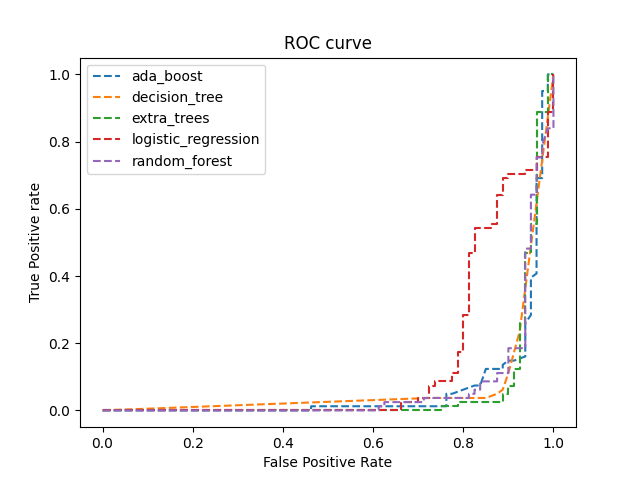
\includegraphics[scale=0.6]{fakeexp1/roccurves.png}
\caption{ROC Curves of predictions}
\end{figure}
The AUC ROC is low.


\subsection{Experiment 3}
For this experiment, we train on BuzzFeed then:
\begin{enumerate}
\item test on BuzzFeed
\item test on FA-KES
\end{enumerate}


\subsection{Train on BuzzFeed, Test on BuzzFeed}
\subsubsection{Mean Empirical Risks}
\begin{figure}[H]
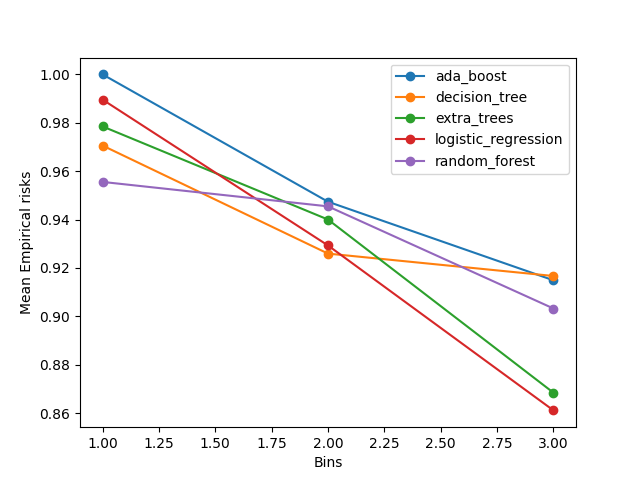
\includegraphics[scale=0.6]{fakeexp3buzz/meanempiricalrisks.png}
\caption{plot that shows the mean empirical risks across the 3 bins}
\end{figure}

\subsubsection{Precision at Top K}
\begin{figure}[H]
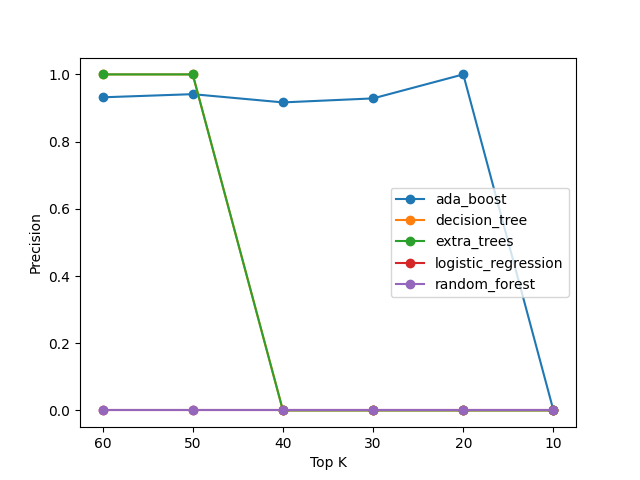
\includegraphics[scale=0.6]{fakeexp3buzz/precisionstopK.png}
\caption{Precison at Top K instances that have the highest risk scores}
\end{figure}
Precision is decreasing for extra trees and ada boost as the number of Top K decreases. This is good. It means at the top K instances that have the highest risk of being Fake, the precision is high, and as the risk score decreases precision decreases.

The random forest model is not good.

\subsection{Recall at Top K}
\begin{figure}[H]
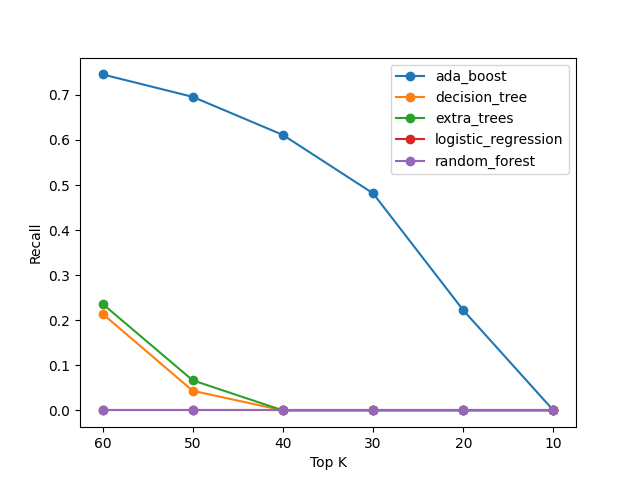
\includegraphics[scale=0.6]{fakeexp3buzz/recallstopK.png}
\caption{Recall at Top K instances that have the highest risk scores}
\end{figure}
Recall is not increasing as K decreases. This is not really good.

\subsection{Jaccard Similarity at Top K}
\begin{figure}[H]
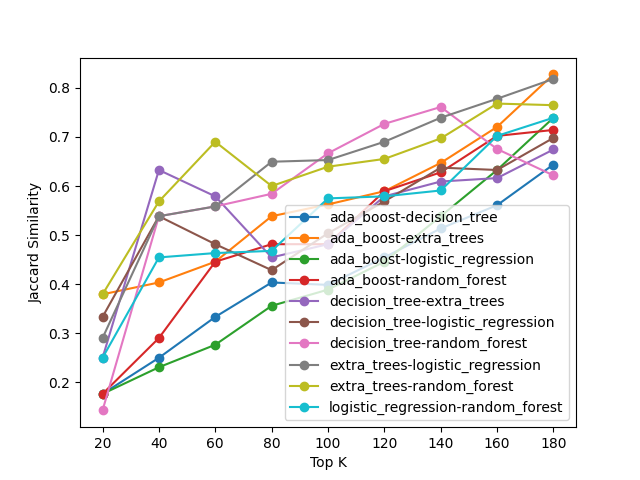
\includegraphics[scale=0.6]{fakeexp3buzz/jaccardtopK.png}
\caption{Jaccard Similarity at Top K instances that have the highest risk scores}
\end{figure}


\subsection{Train on BuzzFeed, Test on FA-KES}
\subsubsection{Mean Empirical Risks}
\begin{figure}[H]
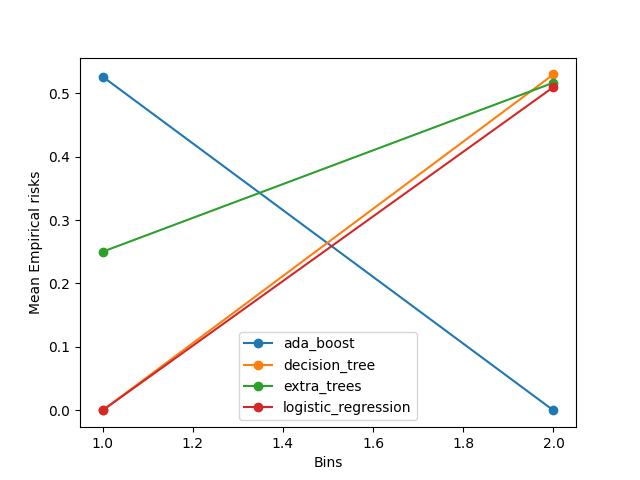
\includegraphics[scale=0.6]{fakeexp3fakes/meanempiricalrisks.png}
\caption{plot that shows the mean empirical risks across the 2 bins}
\end{figure}

Its good that the mean empirical risks for extra trees, decision tree, and logistic regression is increasing, but we cannot do our judgment with 2 bins only. The \textbf{bins problem must be solved for better assessment}

\subsubsection{Precision at Top K}
\begin{figure}[H]
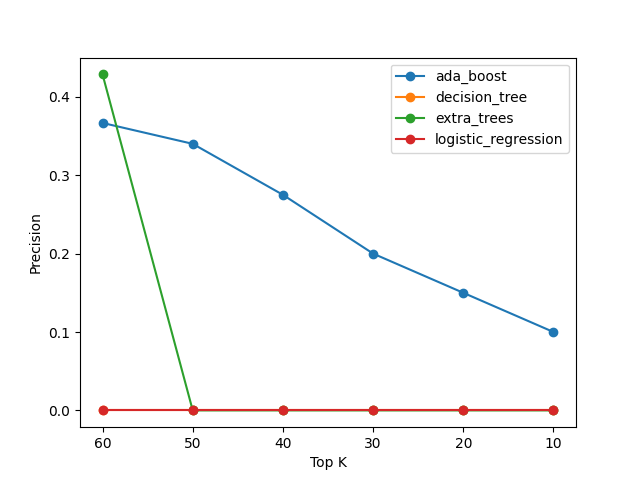
\includegraphics[scale=0.6]{fakeexp3fakes/precisionstopK.png}
\caption{Precison at Top K instances that have the highest risk scores}
\end{figure}
Precision is decreasing for extra trees and ada boost as the number of Top K decreases. This is good. It means at the top K instances that have the highest risk of being Fake, the precision is high, and as the risk score decreases precision decreases.

The logistic regression model is not good.

\subsection{Recall at Top K}
\begin{figure}[H]
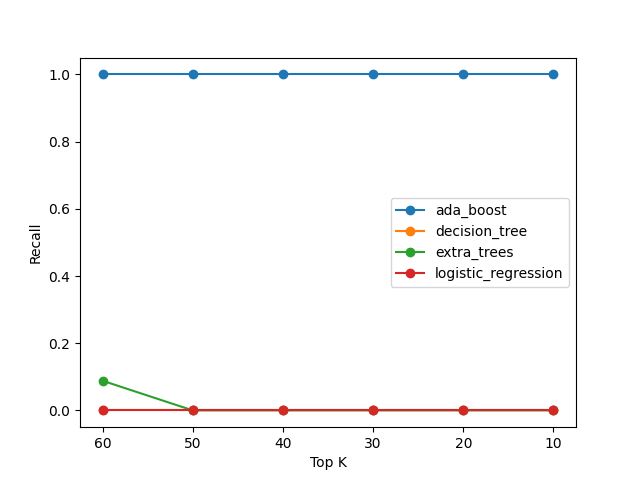
\includegraphics[scale=0.6]{fakeexp3fakes/recallstopK.png}
\caption{Recall at Top K instances that have the highest risk scores}
\end{figure}
Recall is not increasing as K decreases. This is not really good.

\subsection{Jaccard Similarity at Top K}
\begin{figure}[H]
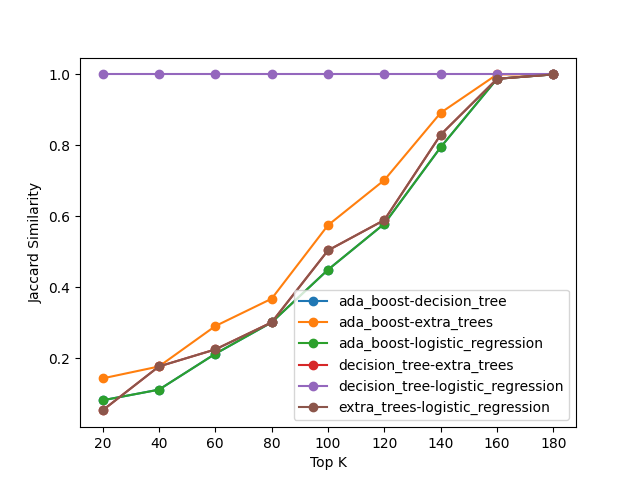
\includegraphics[scale=0.6]{fakeexp3fakes/jaccardtopK.png}
\caption{Jaccard Similarity at Top K instances that have the highest risk scores}
\end{figure}


\end{document}